\chapter{IMPLEMENTASI DAN PENGUJIAN}

Pada bab ini akan menjelaskan tentang implementasi program, pengujiannya dan masalah yang dihadapi

\section{Implementasi}
\subsection{Lingkungan Implementasi}
Berikut adalah spesifikasi \textit{laptop} yang digunakan:
\begin{itemize}
    \item \textit{Processor}: Intel Core i7-6700HQ
    \item \textit{Memory}: 16384 MB RAM @2300 MHz
    \item \textit{Operating System}: Windows 10 Pro 64-bit
\end{itemize}


Berikut adalah spesifikasi perangkat lunak yang digunakan untuk implementasi program:
\begin{itemize}
    \item IDE: Ecplipse verison 4.12.0
    \item Bahasa Pemograman: Java
    \item Java Library version : Java 1.8.0 191
\end{itemize}

Berikut adalah spesifikasi node sensor yang digunakan untuk implementasi program:
\begin{itemize}
    \item Nama sensor: Preon32
    \item Processor: Cortex-M3
    \item Operating System: PreonVM
    \item Penyimpanan Sistem: 64 kByte SRAM
    \item Penyimpnan Data: 250 kByte Flash
    \item Pita Frekuensi: 2400.0 - 2483.5 MHz
    \item Jangkauan: 250 meter (luar ruangan) dan 30 meter (dalam ruangan)
    \item Sensor-sensor: Sensor getaran, sensor cahaya, sensor suhu, sensor kelembaban, dan sensor tekanan udara
\end{itemize}

\subsection{Hasil Implementasi Kelas}

Berdasarkan pembahasan pada bab 4, terdapat beberapa kelas yang diimplementasi pada \textit{sensor node} yaitu kelas \textit{Accelerometer, SensorManager, BaseStation}. Kelas-kelas yang diimplementasi pada \textit{sensor node} ini akan diatur oleh kelas \textit{SensorManager} dan \textit{BaseStaion} jika sensor node berperan sebagai \textit{BaseStation}. Selain dari kelas yang telah disebut, terdapat kelas yang telah diimplementasi di komputer sebagai penghubung antara \textit{base station} dengan komputer dan juga digunakan untuk melakukan proses perhitungan pada hasil sense.

\subsubsection{Kelas Accelerometer}
Kelas ini digunakan untuk mengatur dan menginisialisasi objek ADXL345 dan GPIO agar dapat mengatur sensor \textit{accelerometer} terdapat pada sensor node. Terdapat metode \textit{init} yang digunakan sebagai konstruktor dari kelas \textit{Accelerometer}. Metode \textit{sensing} yang digunakan untuk melakukan pengukuran dan mengubah pengukuran ke dalam satuan gravitasi. Kode program kelas ini dapat dilihat pada lampiran \ref{lamp:A} bagian \ref{lamp:accelerometer}.


\subsubsection{Kelas SensorManager}
Kelas ini digunakan sebagai main class pada sensor node. Saat sensor node dijalankan, atribut-atribut akan diinisialisasi dan metode \textit{starts} dijalankan. Metode \textit{starts} akan menginisalisasi \textit{Transciever}, \textit{RadioDriver} yang berfungsi untuk komunikasi antar sensor node dan \textit{FrameIO} berfungsi sebagai pengiriman atau penerimaan pesan. 

Kemudian metode \textit{recieve} dijalankan, sensor node akan menerima pesan-pesan yang memiliki arti tertentu. Saat node sensor menerima pesan '@1', maka metode \textit{recieve} akan menyamakan waktu dari pesan yang telah dikirim serta dengan mengirimkan status 'ONLINE' ke \textit{BaseStation}. Jika sensor node menerima pesan '@2', maka sensor node akan membuat \textit{thread} baru yang akan digunakan untuk memulai proses \textit{sensing}. Hasil sensing kemudian akan dikirimkan dengan metode \textit{send} menuju \textit{BaseStation}. Saat sensor node menerima pesan '@3', sensor node akan berhenti melakukan sensing dan mengirimkan pesan ke \textit{BaseStation} apabila \textit{sensing} telah berhenti. Saat sensor node menerima pesan '@4', sensor node akan menghentikan program. Kode program dapat dilihat pada lampiran \ref{lamp:A} bagian \ref{lamp:sensorManager}

\subsubsection{Kelas BaseStation}
Kelas ini digunakan sebagai main class pada sensor node yang berperan menjadi \textit{BaseStation} dimana merupakan penghubung secara langsung ke komputer. Kelas ini akan menginisialisasi \textit{USART} yang bertujuan untuk menerima pesan dan juga mengirim pesan dari pengguna komputer. Setelah \textit{USART} terinisialisasi, kelas ini akan memulai \textit{thread} baru dan metode \textit{starts} dijalankan. Metode \textit{starts} akan menginisalisasi \textit{Transciever}, \textit{RadioDriver} yang berfungsi untuk komunikasi antar sensor node dan \textit{FrameIO} dan memulai \textit{thread} baru untuk menerima input dari komputer. Setelah \textit{BaseStation} menerima pesan dari komputer, \textit{BaseStation} akan mengirimkan pesan menuju ke alamat node sensor yang terhubung yang disimpan pada atribut \textit{connectedNode} dengan \textit{USART}. Metode \textit{recieve} telah diimplementasi dan dapat dilihat pada Listing \ref{recieve_base}.   
\begin{lstlisting}[language=Java, caption=Metode recieve(), label=recieve_base]
public static void recieve(final FrameIO fio){
	while(true) {
		Frame frame = new Frame();
		try {
			fio.receive(frame);
			byte[] content = frame.getPayload();
			String str = new String(content, 0, content.length);
			if(str.trim().charAt(0)=='1') {
				usart.write(str.getBytes());
				usart.flush();
			}
			else if(str.trim().charAt(0)=='2') {
				usart.write(str.getBytes());
				usart.flush();
			}
			else if(str.trim().charAt(0)=='3') {
				usart.write(str.getBytes());
				usart.flush();
			}
			else if(str.trim().charAt(0)=='4') {
				usart.write(str.getBytes());
				usart.flush();
			}
		}
		catch(USARTException e) {
			
		}
		catch(IOException e) {
			
		}
	}
}
\end{lstlisting}


Kode program dari kelas ini dapat dilihat pada lampiran \ref{lamp:A} bagian \ref{lamp:baseStation}.


Selain dari kelas yang diimplementasikan di sensor node, terdapat juga kelas-kelas yang diimplementasikan pada komputer pengguna yaitu \textit{Complex, FFT, GraphAmplitude, GraphFrequency, SampleData, Tester, dan Visual}.

\subsubsection{Kelas Complex}
Kelas ini digunakan untuk merepresentasikan bilangan kompleks. Pada kelas ini terdapat konstruktor, setter dan getter untuk setiap atribut dan beberapa metode yang digunakan untuk melakukan operasi bilangan kompleks. Metode \textit{add} digunakan untuk melakukan operasi penjumlahan pada bilangan kompleks, metode \textit{minus} digunakan untuk melakukan opersi pengurangan pada bilangan kompleks, metode \textit{multiplication} digunakan untuk melakukan operasi perkalian pada bilangan kompleks dan metode \textit{absolute} digunakan untuk memutlakkan bilangan kompleks. Metode \textit{toString} digunakan untuk menjadikan bilangan kompleks ke dalam bentuk \textit{String}. Kode program pada kelas ini dapat dilihat pada lampiran \ref{lamp:A} bagian \ref{lamp:complex}.

\subsubsection{Kelas FFT}
Pada kelas FFT terdapat metode bitReverse yang memiliki fungsi untuk melakukan \textit{in bit reverse order} pada input dari algoritma FFT. Metode bitReverse yang telah diimplementasi dapat dilihat pada listing \ref{bitReverse}.
\begin{lstlisting}[language=Java, caption=Metode bitReverse(), label=bitReverse]
public int bitReverse(int banyak, int bit) {
	if(banyak==0) {
		return 0;
	}
	
	String temp = Integer.toBinaryString(banyak);
	if(temp.length()<bit) {
		int ct = bit - temp.length();
		for(int i=0; i<ct; i++) {
			temp = "0" + temp;
		}
	}
	
	int hasil = 0;
	for(int i = temp.length()-1; i>=0; i--) {
		if(temp.charAt(i) == '1') {
			hasil += Math.pow(2, i);
		}
	}
	return hasil;
}
\end{lstlisting}

Terdapat juga metode FFT yang berfungsi untuk melakukan algoritma FFT. Metode fft yang telah diimplementasi dapat dilihat pada listing \ref{fft}.
\begin{lstlisting}[language=Java, caption=Metode fft(), label=fft]
public Complex[] fft(Complex[] input) {
	int bit = (int) (Math.log(input.length) / Math.log(2));
	Complex[] orderFinal = new Complex[input.length];
	for(int i=0; i<input.length; i++) {
		int order = bitReverse(i,bit);
		orderFinal[i] = input[order];
	}
	
	for(int i=2; i<= orderFinal.length; i=i*2 ) {
		for(int j=0; j<orderFinal.length; j +=i) {
			for(int k=0; k<i/2; k++) {
				Complex awal = orderFinal[j+k];
				Complex akhir = orderFinal[j+k+(i/2)];
				
				double weight = (-2 * Math.PI * k)/ (double) i;
				Complex exponential = (new Complex(Math.cos(weight), Math.sin(weight)).multiplication(akhir));
				
				orderFinal[j+k] = awal.add(exponential);
				orderFinal[j+k+(i/2)] = awal.minus(exponential);
			}
		}
	}
	return orderFinal;
}
\end{lstlisting}
Kode program secara keseluruhan pada kelas FFT dapat dilihat pada lampiran \ref{lamp:A} bagian \ref{lamp:fft}.

\subsubsection{Kelas StartChart}
Kelas ini digunakan untuk membuat window hasil grafik yang ditampilkan ke \textit{user}. Kelas ini terdapat beberapa metode yaitu \textit{getScene()} dan \textit{addData()}. Hasil implementasi metode dapat dilihat pada listing \ref{getScene} dan \ref{addData}.
\begin{lstlisting}[language=Java, caption=Metode getScene(), label=getScene]
    public Scene getScene() {
        charts.add(new ChartAmplitude(this.getSample(), this.getData(), sensorId));
        this.getSample().setRender(charts.get(0));
        charts.add(new ChartFrequency(this.getSample(), this.getData(), sensorId));
        this.getData().setRender(charts.get(1));
        AnchorPane ap = new AnchorPane();
        int i = 0;
        int height = 400;
        int width = 600;
        for (Chart chart : charts) {
            LineChart lc = chart.getChart();
            lc.relocate(0, height * i);
            i++;
            ap.getChildren().add(lc);
            lc.setMinSize(width, height);
            lc.setMaxSize(width, height);
        }
        return new Scene(ap, width, i * height);
    }
\end{lstlisting}

\begin{lstlisting}[language=Java, caption=Metode addData(), label=addData]
    public void addData(String[] hasil){
        if (hasil[0].charAt(0) == '2') {
            // Sample Data
            this.getSample().addX(Double.parseDouble(hasil[1]));
            this.getSample().addY(Double.parseDouble(hasil[2]));
            this.getSample().addZ(Double.parseDouble(hasil[3]));

            // Perhitungan FFT
            FFT computeFFT = new FFT(this.getSample());
            computeFFT.convertComplex();
            Complex[] tempRes1 = computeFFT.fft(computeFFT.xComplex);
            Complex[] tempRes2 = computeFFT.fft(computeFFT.yComplex);
            Complex[] tempRes3 = computeFFT.fft(computeFFT.zComplex);
            double t1 = 0, t2 = 0, t3 = 0;
            DecimalFormat df = new DecimalFormat("#.####");
            for (int i = 0; i < tempRes1.length; i++) {
                t1 += tempRes1[i].absolute();
                t2 += tempRes2[i].absolute();	
                t3 += tempRes3[i].absolute();
            }
            t1/= tempRes1.length;
            t2/= tempRes2.length;
            t3/= tempRes3.length;
            System.out.printf("%f %f %f\n",t1,t2,t3);
            this.getData().setX(Double.parseDouble(df.format(t1)));
            this.getData().setY(Double.parseDouble(df.format(t2)));
            this.getData().setZ(Double.parseDouble(df.format(t3)));
            
        }
    }
\end{lstlisting}
Kode program secara keseluruhan pada kelas StartChart dapat dilihat pada lampiran \ref{lamp:A} bagian \ref{lamp:startChart}.

\subsubsection{Kelas ChartAmplitude dan ChartFrequency}
Kelas ini berfungsi untuk menampilkan LineChart yang akan ada pada window dari kelas StartChart. Kelas ini akan menampilkan nilai amplitudo pada LineChart(ChartAmplitude) dan menampilkan nilai frekuensi pada Line Chart(ChartFrequency). Kelas ini memiliki beberapa metode yaitu \textit{getChart()} dan \textit{render()}. Hasil implementasi \textit{getChart()} dan \textit{render()} pada kelas ChartAmplitude dapat dilihat pada listing \ref{getChartAmplitude} dan \ref{renderAmplitude}. Hasil implementasi \textit{getChart()} dan \textit{render()} pada kelas ChartFrequency dapat dilihat pada listing \ref{getChartFrequency} dan \ref{renderFrequency}.

\begin{lstlisting}[language=Java, caption=Metode getChart() (ChartAmplitude), label=getChartAmplitude]
    public LineChart<String, Number> getChart() throws IOException {
        final CategoryAxis x = new CategoryAxis(); // buat sumbu x (waktu)
        final NumberAxis y = new NumberAxis(); // buat sumbu y (hasil sensor)

        x.setLabel("Time");
        x.setAnimated(false);
        y.setLabel("Value (g)");
        y.setAnimated(false);

        // bikin line chart
        lineChart = new LineChart<>(x, y);
        lineChart.setAnimated(false);

        series1.setName("Sumbu X");
        series2.setName("Sumbu Y");
        series3.setName("Sumbu Z");
        
        // add series to chart
        lineChart.getData().add(series1);
        lineChart.getData().add(series2);
        lineChart.getData().add(series3);

        // setup scene

        // setup executor to put data periodically
        scheduledExecutorService = Executors.newSingleThreadScheduledExecutor();

        render();
        return this.lineChart;
    }
\end{lstlisting}

\begin{lstlisting}[language=Java, caption=Metode render() (ChartAmplitude), label=renderAmplitude]
    public void render() throws IOException{
    	
    	Platform.runLater(new Runnable() {
			
			@Override
			public void run() {

		    	Date now = new Date();
		        lineChart.setTitle("Grafik Amplitudo " +sensorId);
		        
		        try {
					String baris = sensorId+", "+getX()+", "+getY()+", "+getZ();
					writer.write(baris);
					writer.newLine();
					writer.flush();
				}
				catch(Exception e) {
					e.getMessage();
				}
		        // taro random number dengan waktu skrng
		        series1.getData().add(new XYChart.Data<>(simpleDateFormat.format(now), getX()));
		        series2.getData().add(new XYChart.Data<>(simpleDateFormat.format(now), getY()));
		        series3.getData().add(new XYChart.Data<>(simpleDateFormat.format(now), getZ()));
		        if (series1.getData().size() > WINDOW_SIZE) {
		            series1.getData().remove(0);
		            series2.getData().remove(0);
		            series3.getData().remove(0);
		        }
			}
		});
    }
\end{lstlisting}

\begin{lstlisting}[language=Java, caption=Metode getChart() (ChartFrequency), label=getChartFrequency]
    public LineChart<String, Number> getChart() {
        final CategoryAxis x = new CategoryAxis(); // buat sumbu x (waktu)
        final NumberAxis y = new NumberAxis(); // buat sumbu y (hasil sensor)

        x.setLabel("Time");
        x.setAnimated(false);
        y.setLabel("Value (Hz)");
        y.setAnimated(false);

        // bikin line chart
        lineChart = new LineChart<>(x, y);
        lineChart.setAnimated(false);

        // buat nampilin datanya
        series1.setName("Sumbu X");

        series2.setName("Sumbu Y");

        series3.setName("Sumbu Z");

        // add series to chart
        lineChart.getData().add(series1);
        lineChart.getData().add(series2);
        lineChart.getData().add(series3);

        render();
        return this.lineChart;

    }
\end{lstlisting}

\begin{lstlisting}[language=Java, caption=Metode render() (ChartFrequency), label=renderFrequency]
    public void render() {
    	Platform.runLater(new Runnable() {
			
			@Override
			public void run() {
				lineChart.setTitle("Grafik Frekuensi " +sensorId);
		        Date now = new Date();
		        
		        try {
					String baris = sensorId+", "+dataFrequency.X+", "+dataFrequency.Y+", "+dataFrequency.Z;
					writer.write(baris);
					writer.newLine();
					writer.flush();
				}
				catch(Exception e) {
					e.getMessage();
				}
		        series1.getData()
		                .add(new XYChart.Data<>(simpleDateFormat.format(now), dataFrequency.X));
		        series2.getData()
		                .add(new XYChart.Data<>(simpleDateFormat.format(now), dataFrequency.Y));
		        series3.getData()
		                .add(new XYChart.Data<>(simpleDateFormat.format(now), dataFrequency.Z));
		        tempX = dataFrequency.X;
		        tempY = dataFrequency.Y;
		        tempZ = dataFrequency.Z;
		        if (series1.getData().size() > WINDOW_SIZE) {
		            series1.getData().remove(0);
		            series2.getData().remove(0);
		            series3.getData().remove(0);
		        }
			}
		});
    }
\end{lstlisting}
Kode program secara keseluruhan pada kelas ChartAmplitude dan ChartFrequency dapat dilihat pada lampiran \ref{lamp:A} bagian \ref{lamp:startChart}.

\subsubsection{Kelas RenderChart}
Kelas ini merupakan \textit{interface class} yang akan digunakan pada kelas ChartAmplitude dan ChartFrekuensi. Kode program secara keseluruhan dapat dilihat pada \ref{lamp:A} bagian \ref{lamp:renderChart}.

\subsubsection{SampleData}
Kelas ini berfungsi untuk membuat sampel data berdasarkan hasil sensing. Pada kelas ini terdapat beberapa atribut yang digunakan untuk menyimpan hasil sensing. Kode program ini dapat dilihat pada lampiran \ref{lamp:A} bagian \ref{lamp:sampleData}.

\subsubsection{Sensor}
Kelas ini merupakan main class dari komputer pengguna. Kelas ini digunakan sebagai penghubung komunikasi dan memberikan perintah kepada BaseStation. Sebelum kelas ini dijalankan, BaseStation harus terlebih dahulu terhubung dengan komputer pengguna melalui USB PORT.

Saat kelas ini dijalankan, komputer pengguna dan BaseStation akan diinisialisasi dengan metode \textit{context\_set} dan BaseStation melakukan sinkronisasi waktu dengan komputer dengan metode \textit{time\_synchronize}. Setelah itu dibuat objek Preon32Helper untuk menjalankan module pada BaseStation dan mengatur koneksi komunikasi dengan BaseStation.  

Kemudian kelas ini akan menampilkan 4 pilihan yang dapat dipilih oleh penggunaa yaitu "Check Online Node Status", "Start Sensing", "Stop Sensing", dan "Exit Program". Jika pengguna memasukkan angka '1', maka aplikasi akan menampilkan node-node sensor yang berstatus "ONLINE" beserta waktunya. Jika pengguna memasukkan angka '2', maka aplikasi akan menampilkan status "Sensing..." dan menampilkan grafik dari setiap node sensor. Jika pengguna memasukkan angka '3', maka aplikasi yang sedang dalam status sensing akan berhenti. Jika pengguna memasukan angka '4', maka aplikasi akan berhenti. Kode program dapat dilihat pada lampiran \ref{lamp:A} bagian \ref{lamp:sensor}.

\subsection{Hasil Implementasi Antar Muka Visualisasi Hasil \textit{Sense}}
Berikut contoh hasil dari implementasi antar muka visualisasi hasil \textit{sense} menggunakan \textit{library} dari \textit{JavaFX}:
\begin{figure}[H] 
	\centering  
	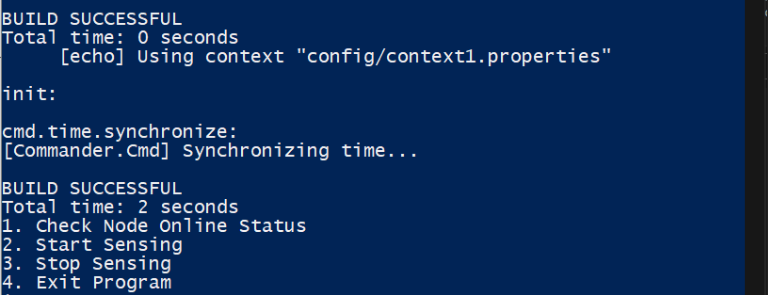
\includegraphics[scale=1]{Gambar/Hasil Sensing/visualisasi.PNG}
	\caption[Tampilan awal aplikasi]{Tampilan awal aplikasi}
	\label{fig:tampilan awal} 
\end{figure}

\begin{figure}[H] 
	\centering  
	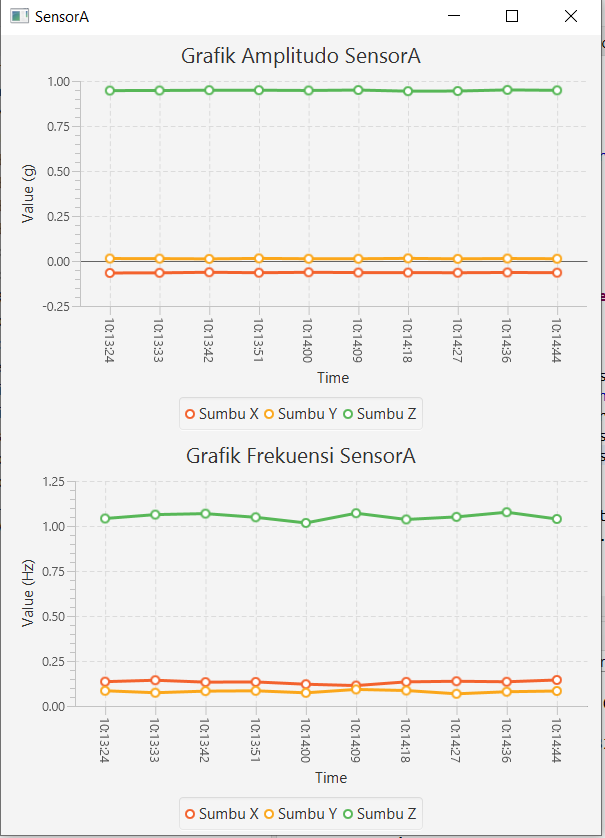
\includegraphics[scale=1]{Lampiran/HasilPengujian/sensorA_starRooftop.PNG}
	\caption[Grafik hasil implementasi visualisasi hasil \textit{sense}]{Grafik hasil implementasi visualisasi hasil \textit{sense}}
	\label{fig:tampilan_sensing} 
\end{figure}

Pada tampilan awal (Gambar \ref{fig:tampilan awal}), pengguna perlu memilih \textit{option} \textit{Sense}. Tampilan hasil visualisasi hasil \textit{sense} akan muncul setelah sensor node mengirimkan hasil \textit{sense}. Grafik visualisasi akan menunjukan amplitudo dan frekuensi dari sensor yang dapat dilihat pada (Gambar \ref{fig:tampilan_sensing}).

\section{Pengujian}
Pengujian dilakukan dengan menggunakan dua metode, yaitu pengujian fungsional dan pengujian eksperimental

\subsection{Pengujian Fungsional}
Pengujian dilakukan dengan menjalankan aplikasi dengan \textit{Command Line Interface}. Tampilan utama ketika aplikasi dijalankan dapat dilihat pada Gambar \ref{fig:tampilan awal2}
\begin{figure}[H] 
	\centering  
	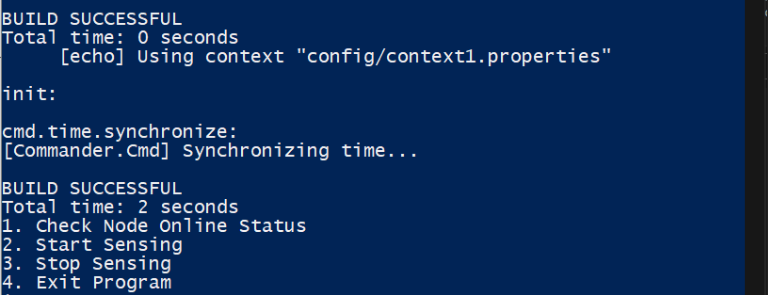
\includegraphics[scale=1]{Gambar/Hasil Sensing/visualisasi.PNG}
	\caption[Tampilan awal aplikasi]{Tampilan awal aplikasi}
	\label{fig:tampilan awal2} 
\end{figure}

Fitur-fitur yang terdapat pada aplikasi adalah sebagai berikut:
\begin{itemize}
    \item Check Online Node Status
    
    Fitur ini berfungsi untuk menampilkan sensor node - sensor node yang sedang menyala dan menyamakan waktu pada sensor node dengan waktu yang ada pada komputer pengguna. Untuk menjalankan fitur ini, pengguna memasukkan angka '1' dan menunggu hasil yang ditampilkan seperti pada Gambar \ref{fig:check_node}.
    
    \begin{figure}[H] 
    	\centering  
    	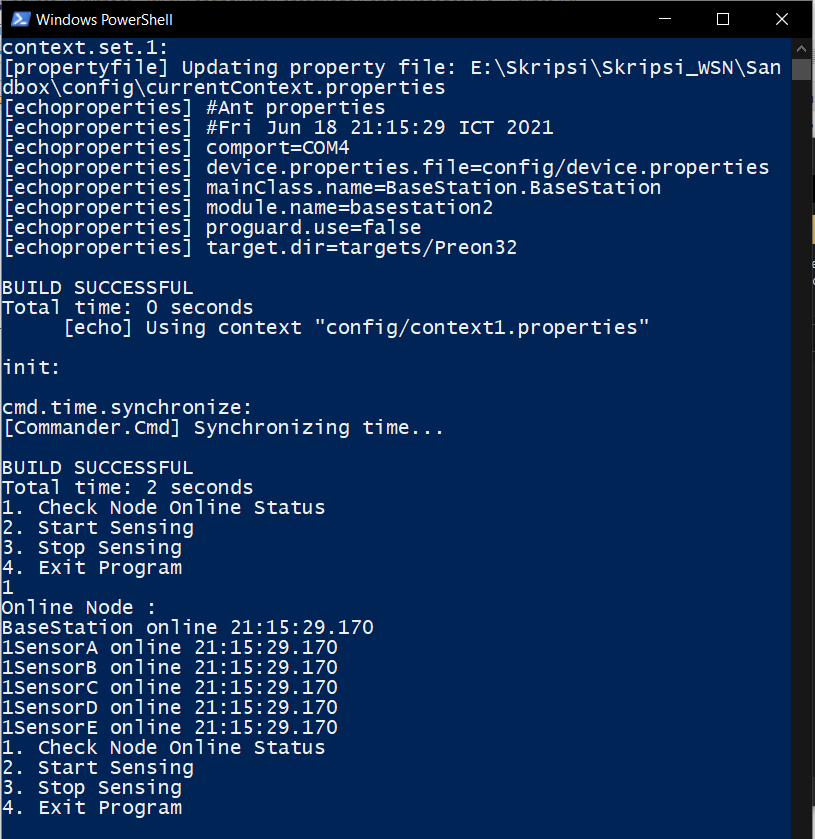
\includegraphics[scale=0.8]{Lampiran/HasilPengujian/fungsional1.PNG}
    	\caption[Pengujian "Check Node Online Status"]{Pengujian "Check Node Online Status"}
    	\label{fig:check_node} 
    \end{figure}
    
    \item Start Sensing
    
    Fitur ini berfungsi untuk memberikan perintah kepada sensor node - sensor node yang sedang menyala untuk melakukan \textit{sensing}. Saat pengguna memasukkan angka '2', aplikasi akan menampilkan grafik hasil \textit{sensing} dan grafik frekuensi yang akan terus diperbaharui. Berikut tampilan yang tampil setelah pengguna memasukkan angka '2' seperti pada Gambar \ref{fig:start_sensing}.
    
    \begin{figure}[H] 
    	\centering  
    	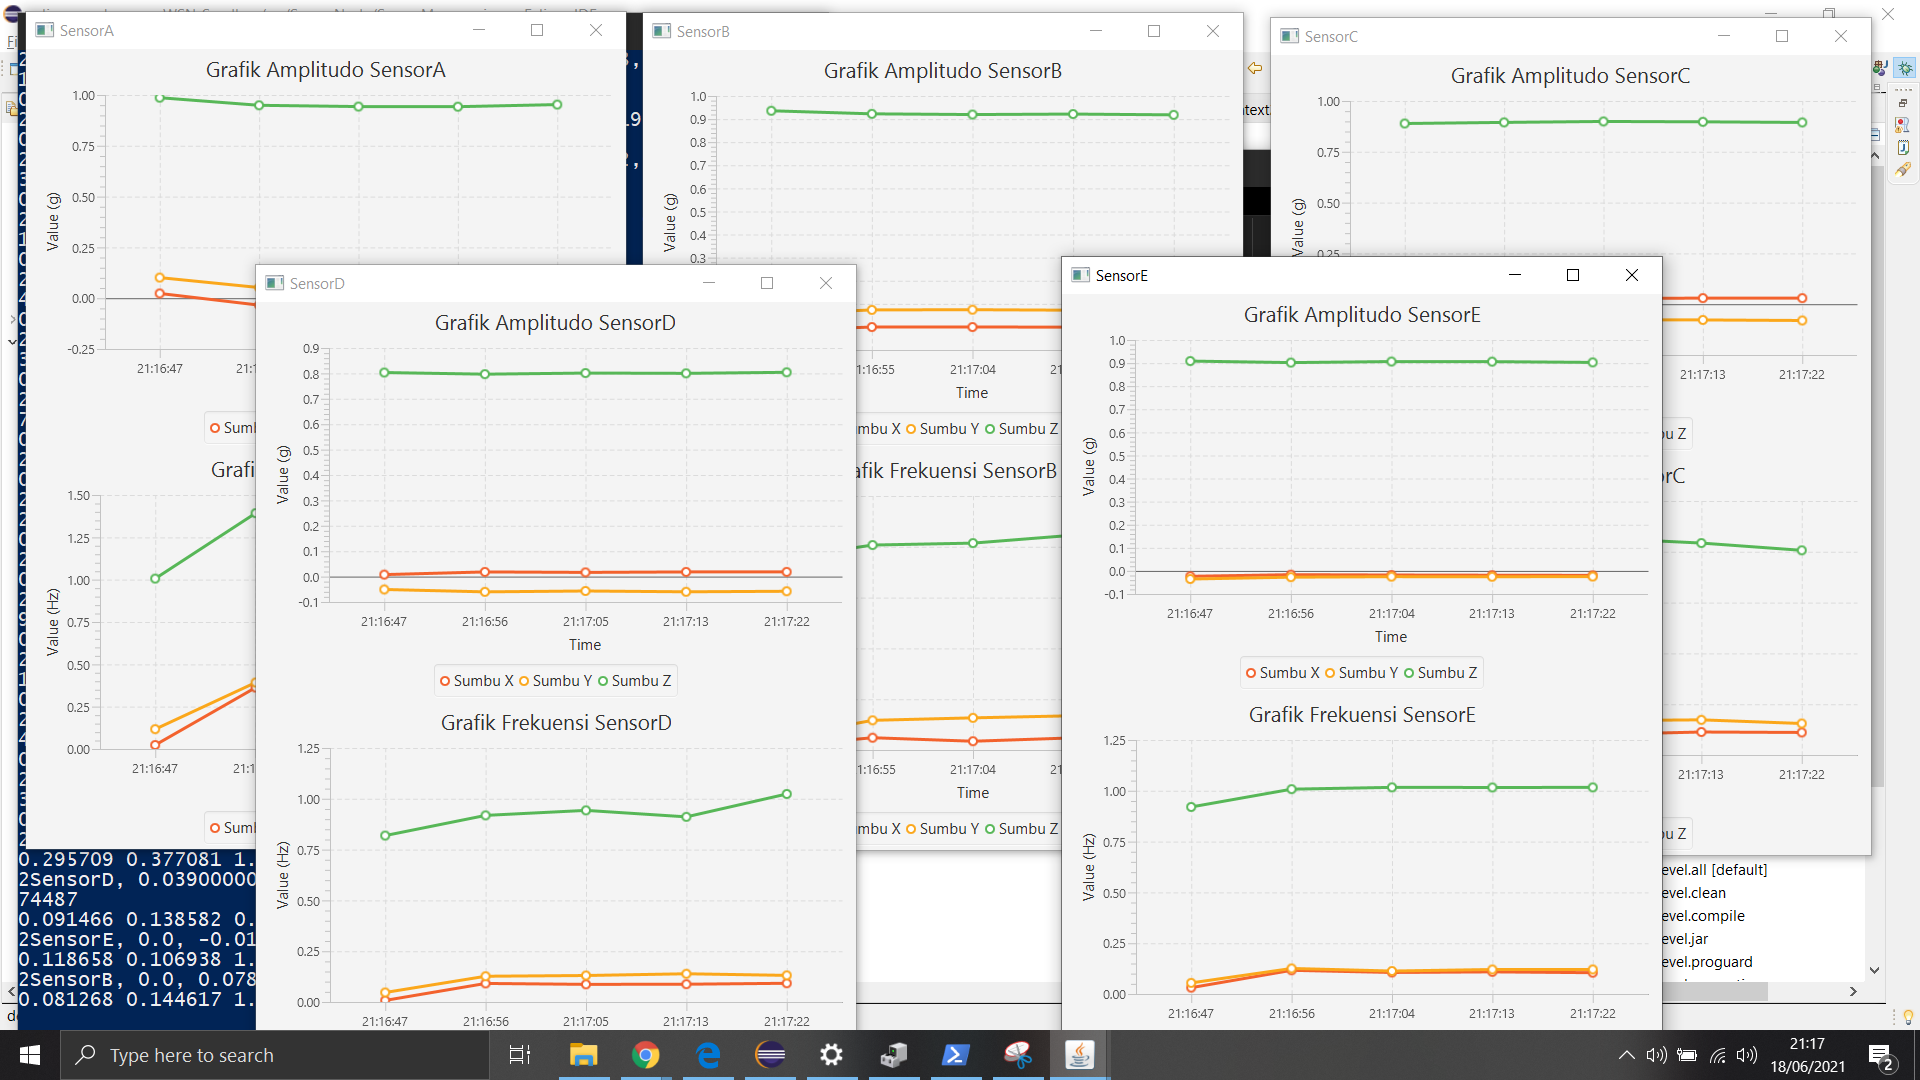
\includegraphics[scale=0.24]{Gambar/Hasil Sensing/fungsional2.png}
    	\caption[Pengujian "Start sensing"]{Pengujian "Start sensing"}
    	\label{fig:start_sensing} 
    \end{figure}
    
    Saat fungsi \textit{start sensing} berjalan, aplikasi tidak akan menerima input selain masukan angka '3' untuk memberhentikan \textit{sensing}. Tampilan jika pengguna memasukkan input selain angka '3' dapat dilihat pada Gambar \ref{fig:in_sensing}.
    
    \begin{figure}[H] 
    	\centering  
    	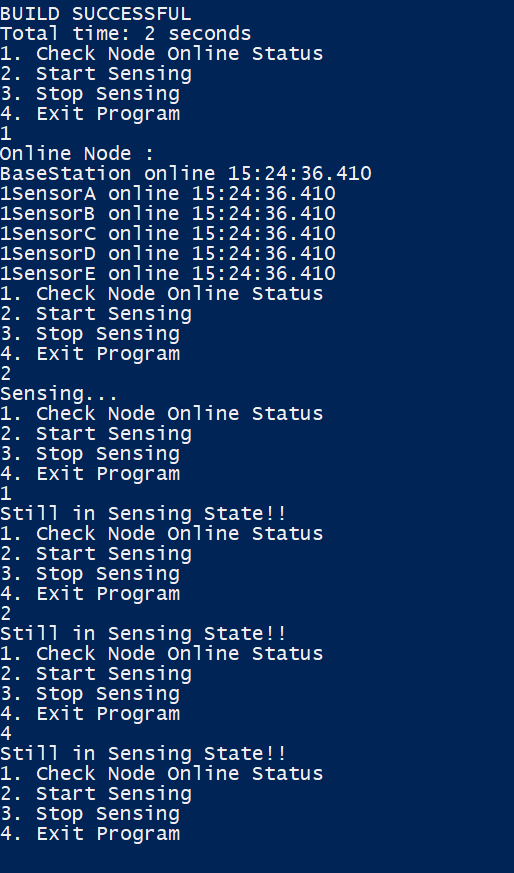
\includegraphics[scale=0.8]{Gambar/Hasil Sensing/instateSensing.PNG}
    	\caption[Pengujian input selain angka '3' saat "Start sensing"]{Pengujian input selain angka '3' saat "Start sensing"}
    	\label{fig:in_sensing} 
    \end{figure}
    
    \item Stop sensing
    
    Fitur ini berfungsi untuk menghentikan sensor node yang sedang melakukan \textit{sensing}. Pengguna harus memasukkan angka '3' saat sensor node sedang \textit{sensing} untuk menjalankan fungsi ini. Tampilan setelah fungsi ini dijalankan dapat dilihat seperti pada Gambar \ref{fig:stop_sensing}.
    
    \begin{figure}[H] 
    	\centering  
    	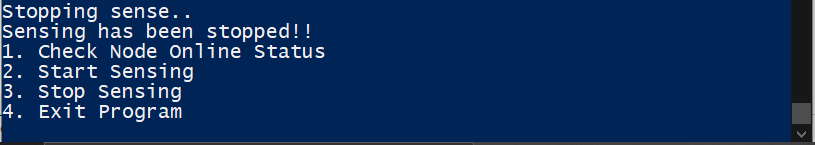
\includegraphics[scale=1]{Lampiran/HasilPengujian/fungsional3.PNG}
    	\caption[Pengujian "Stop sensing"]{Pengujian "Stop sensing"}
    	\label{fig:stop_sensing} 
    \end{figure}
    
    \item Exit Program
    
    Fitur ini berfungsi untuk keluar dari aplikasi. Pengguna harus memasukkan angka '4'saat sensor node tidak dalam keadaan \textit{sensing} untuk menjalankan fungsi ini. Tampilan hasil dari fungsi ini dapat dilihat pada Gambar \ref{fig:exit_program}.
    
    \begin{figure}[H] 
    	\centering  
    	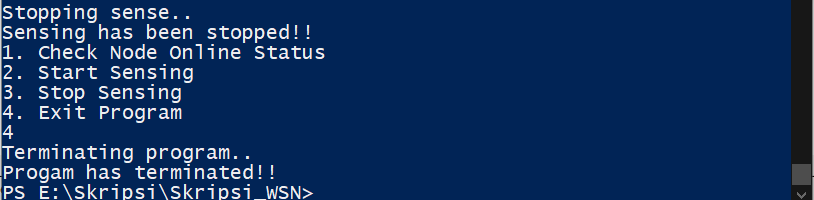
\includegraphics[scale=1]{Lampiran/HasilPengujian/fungsional4.PNG}
    	\caption[Pengujian "Exit Program"]{Pengujian "Exit Program"}
    	\label{fig:exit_program} 
    \end{figure}
\end{itemize}

\subsection{Pengujian Eksperimental}
Pengujian Eksperimental ini dilakukan pada dua tempat, yaitu yang pertama di Mall Paskal 23 Square yang berada di jalan pasir kaliki Bandung. Lokasi spesifik pengujian dilakukan pada lantai 2 outdoor pada mall tersebut. Sedangkan tempat pengujian kedua berada di Universitas Katolik Parahyangan gedung 10 bagian \textit{rooftop}. Sensor node yang digunakan untuk melakukan pengujian berjumlah 6 dengan 1 sensor node sebagai \textit{base station}. Arsitektur WSN yang digunakan adalah \textit{flat} dengan \textit{single-hop} dan \textit{multi-hop}. Pengujian dilakukan untuk melakukan \textit{monitoring} sebuah gedung apakah terjadi sebuah getaran atau tidak. Pengujian ini mengukur frekuensi dari setiap sumbu $x$, $y$, dan $z$ dari \textit{accelerometer}. 

Topologi yang digunakan untuk melakukan pengujian ini adalah topologi \textit{star} (Gambar \ref{fig:star_pengujian} ) dan topologi \textit{tree} (Gambar \ref{fig:tree_pengujian} ). Kedua topologi ini dipilih karena topologi tersebut sudah mencakup 2 jalur komunikasi WSN (\textit{single hop} dan \textit{multi hop}). Topologi star merupakan komunikasi jenis \textit{single hop} karena setiap sensor node terhubung secara langsung dengan \textit{basestation}. Topologi tree merupakan komunikasi jenis \textit{multi hop} karena sensor node tidak terhubung secara langsung dengan \textit{base station}, melainkan sensor node akan terhubung dengan sensor node lainnya yang jaraknya paling dekat.

\begin{figure}[H] 
	\centering  
	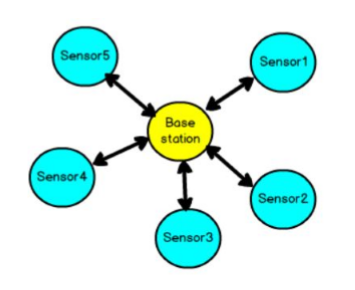
\includegraphics[scale=1]{Gambar/Hasil Sensing/star_pengujian.PNG}  
	\caption[Topologi star yang digunakan (\textit{Single hop}]{Topologi star yang digunakan (\textit{Single hop})}
	\label{fig:star_pengujian} 
\end{figure}

\begin{figure}[H] 
	\centering  
	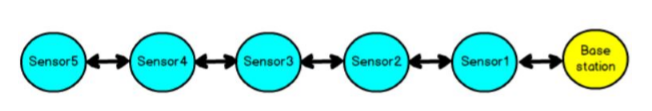
\includegraphics[scale=1]{Gambar/Hasil Sensing/tree_pengujian.PNG}  
	\caption[Topologi tree yang digunakan]{Topologi tree yang digunakan (\textit{Multi hop})}
	\label{fig:tree_pengujian} 
\end{figure}

Skenario-skenario dalam pengujian ini bertujuan untuk melihat kemampuan sensor node untuk melakukan \textit{sensing} dan monitoring getaran yang ditampilkan ke pengguna. Langkah pengujian pada setiap skenario dalam pengujian ini adalah sebagai berikut:
\begin{enumerate}
    \item Peletakan sensor node diatur dengan topologi yang akan diujikan.
    \item Sensor node diletakkan ditempat yang jaraknya cukup jauh pada setiap skenario.
    \item Mengecek status online setiap sensor node melalui komputer.
    \item Memberi perintah \textit{sense} ke setiap sensor node melalui komputer.
    \item Hasil tampilan monitoring getaran akan ditampilkan ke komputer pengguna.
\end{enumerate}
Hasil dari pengujian ini berupa grafik amplitudo akselerasi dari hasil \textit{sensing} dan grafik frekuensi dari setiap node.

\subsubsection{Pengujian di Outdoor lantai 2 Mall Paskal 23 Square}
Pada pengujian ini, sensor akan diletakkan sesuai topologi yang digunakan yaitu topologi star seperti pada Gambar \ref{fig:denah_star_paskal} dan topologi tree seperti pada Gambar \ref{fig:denah_tree_paskal}. Setiap sensor node diberikan jarak antar satu sama lain untuk menunjukan komunikasi setiap sensor node secara nirkabel dan untuk melihat hasil monitoring di lokasi yang berbeda-beda. 

\begin{figure}[H] 
	\centering  
	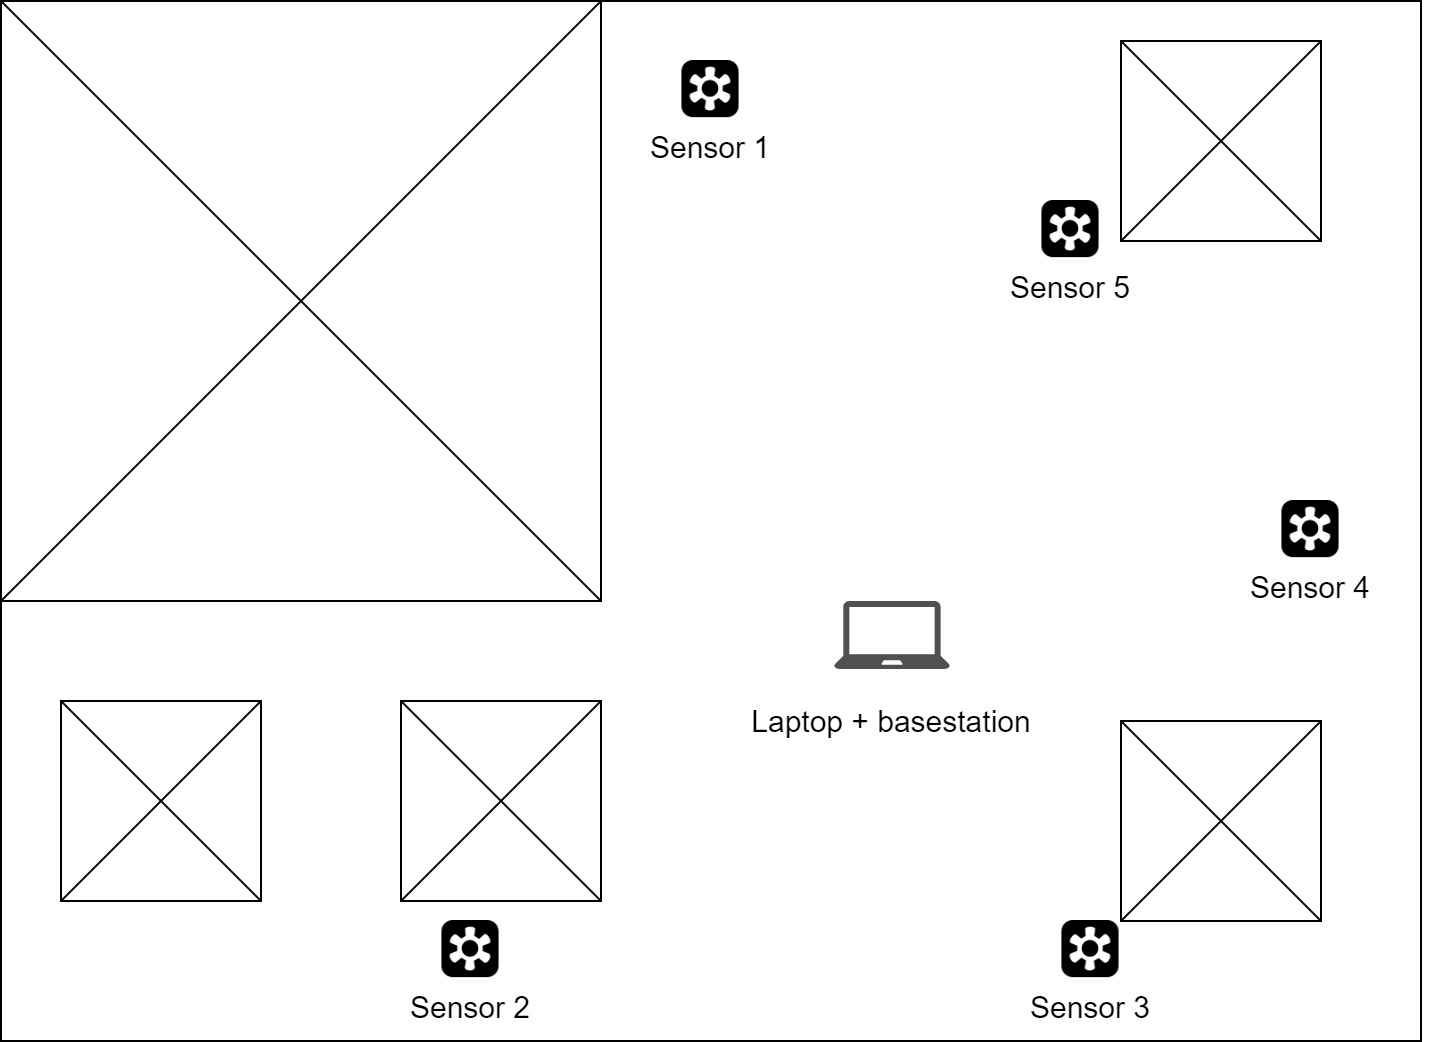
\includegraphics[scale=0.3]{Gambar/Hasil Sensing/Pengujian-Star Paskal 23.jpg}  
	\caption[Denah peletakan sensor node dengan topologi star]{Denah peletakan sensor node dengan topologi star}
	\label{fig:denah_star_paskal} 
\end{figure}

\begin{figure}[H] 
	\centering  
	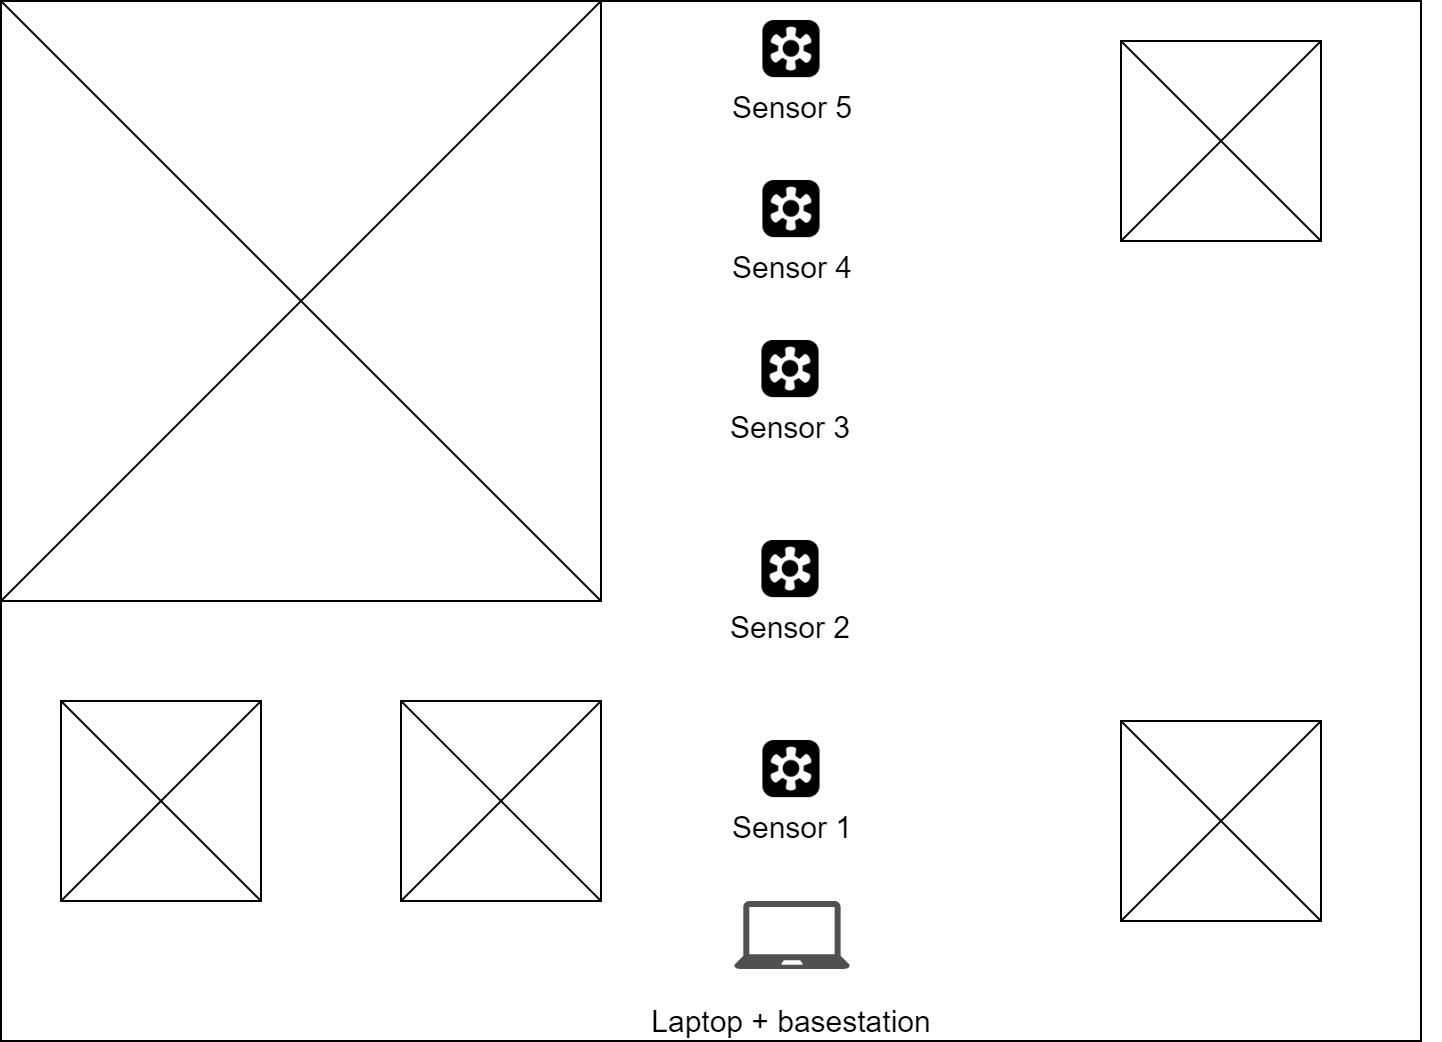
\includegraphics[scale=0.3]{Gambar/Hasil Sensing/Pengujian-Tree Paskal 23.jpg} 
	\caption[Denah peletakan sensor node dengan topologi tree]{Denah peletakan sensor node dengan topologi tree}
	\label{fig:denah_tree_paskal} 
\end{figure}

Pengujian dilakukan saat siang hari dengan cuaca berawan. Hasil grafik dari pengujian dapat dilihat pada lampiran \ref{lamp:B}


\begin{itemize}
    \item Topologi star
    
    \begin{table}[H]
	\centering
	\caption{Tabel hasil getaran yang tertangkap di Mall 23 Paskal Square dengan topologi star}
	\label{star_paskal_tabel}
    	\begin{tabular}{|p{2cm}|p{2cm}|p{3cm}|p{3cm}|p{3cm}|}
    		\hline 
    		Id Sensor & Waktu & Frekuensi pada sumbu $x$ (Hz) & Frekuensi pada sumbu $y$ (Hz) & Frekuensi pada sumbu $z$ (Hz) \\
    		\hline
    		SensorA & 15:07:19 & 1 & 1 & 2.3 \\
    		\hline
    		SensorB & 15:07:28 & 0.15 & 0.15 & 1 \\
    		\hline
    		SensorC & 15:07:26 & 0.10 & 0.20 & 1 \\
    		\hline
    		SensorD & 15:07:08 & 0.35 & 0.30 & 1.25 \\
    		\hline
    		SensorE & 15:07:10 & 0.15 & 0.05 & 1.1 \\
    		\hline
    		SensorA & 15:07:28 & 1.1 & 1.1 & 2.4 \\
    		\hline
    		SensorB & 15:07:37 & 0.15 & 0.15 & 1.01 \\
    		\hline
    		SensorC & 15:07:35 & 0.10 & 0.15 & 1.1 \\
    		\hline
    		SensorD & 15:07:17 & 0.35 & 0.30 & 1.25 \\
    		\hline
    		SensorE & 15:07:20 & 0.15 & 0.05 & 1 \\
    		\hline
    		SensorA & 15:07:37 & 1 & 1.1 & 2.3 \\
    		\hline
    		SensorB & 15:07:46 & 0.15 & 0.16 & 1 \\
    		\hline
    		SensorC & 15:07:44 & 0.10 & 0.15 & 1.1 \\
    		\hline
    		SensorD & 15:07:29 & 0.29 & 0.35 & 1.26 \\
    		\hline
    		SensorE & 15:07:30 & 0.15 & 0.09 & 1.03 \\
    		\hline
    	\end{tabular}
    \end{table}
    
    \pagebreak
    \item Topologi tree
    
    \begin{table}[H]
	\centering
	\caption{Tabel hasil getaran yang tertangkap di Mall 23 Paskal Square dengan topologi tree}
	\label{tree_paskal_tabel}
    	\begin{tabular}{|p{2cm}|p{2cm}|p{3cm}|p{3cm}|p{3cm}|}
    		\hline 
    		Id Sensor & Waktu & Frekuensi pada sumbu $x$ (Hz) & Frekuensi pada sumbu $y$ (Hz) & Frekuensi pada sumbu $z$ (Hz) \\
    		\hline
    		SensorA & 16:45:06 & 0.05 & 0.2 & 1.15 \\
    		\hline
    		SensorB & 16:48:30 & 0.07 & 0.15 & 1.01 \\
    		\hline
    		SensorC & 16:48:30 & 0.20 & 0.30 & 1.1 \\
    		\hline
    		SensorD & 16:48:27 & 0.10 & 0.15 & 0.97 \\
    		\hline
    		SensorE & 16:48:15 & 0.30 & 0.35 & 1.30 \\
    		\hline
    		SensorA & 16:45:15 & 1 & 1 & 2.15 \\
    		\hline
    		SensorB & 16:48:40 & 0.05 & 0.07 & 1 \\
    		\hline
    		SensorC & 16:48:39 & 0.17 & 0.30 & 1.07 \\
    		\hline
    		SensorD & 16:48:36 & 0.10 & 0.10 & 0.95 \\
    		\hline
    		SensorE & 16:48:27 & 0.27 & 0.29 & 1.35 \\
    		\hline
    		SensorA & 16:45:25 & 0.9 & 1.05 & 2.25 \\
    		\hline
    		SensorB & 16:48:49 & 0.07 & 0.17 & 1.01 \\
    		\hline
    		SensorC & 16:48:49 & 0.18 & 0.32 & 1.15 \\
    		\hline
    		SensorD & 16:48:46 & 0.10 & 0.15 & 0.99 \\
    		\hline
    		SensorE & 16:48:38 & 0.26 & 0.30 & 1.32 \\
    		\hline
    	\end{tabular}
    \end{table}
\end{itemize}

Dari tabel \ref{star_paskal_tabel} dan \ref{tree_paskal_tabel} terlihat bahwa hasil frekuensi sensor yang berbeda-beda disebabkan karena perbedaan tempat dan waktu saat melakukan \textit{sensing} sehingga frekuensi yang ditangkap juga nilainya berbeda-beda. Kesimpulan yang didapatkan berdasarkan hasil pengujian adalah frekuensi tertinggi pada sumbu x adalah 1.1 Hz di SensorA pada pengujian topologi star dengan waktu 15:07:28. Frekuensi tertinggi pada sumbu y adalah 1.1 Hz di SensorA pada pengujian topologi star dengan waktu 15:07:28 dan 15:07:37. Frekuensi tertinggi pada sumbu z adalah 2.4 Hz di SensorA pada pengujian topologi star dengan waktu 15:07:28.

\subsubsection{Pengujian di Gedung 10 bagian rooftop Universitas Katolik Parahyangan}

Pada pengujian ini, sensor akan diletakkan sesuai topologi yang digunakan yaitu topologi star seperti pada Gambar \ref{fig:denah_star_rooftop} dan topologi tree seperti pada Gambar \ref{fig:denah_tree_rooftop}. Pengujian dilakukan pada bagian \textit{rooftop} gedung 10 Universitas Katolik Parahyangan. Setiap sensor node diberikan jarak antar satu sama lain untuk menunjukan komunikasi setiap sensor node secara nirkabel dan untuk melihat hasil monitoring di lokasi yang berbeda-beda. 

\begin{figure}[H] 
	\centering  
	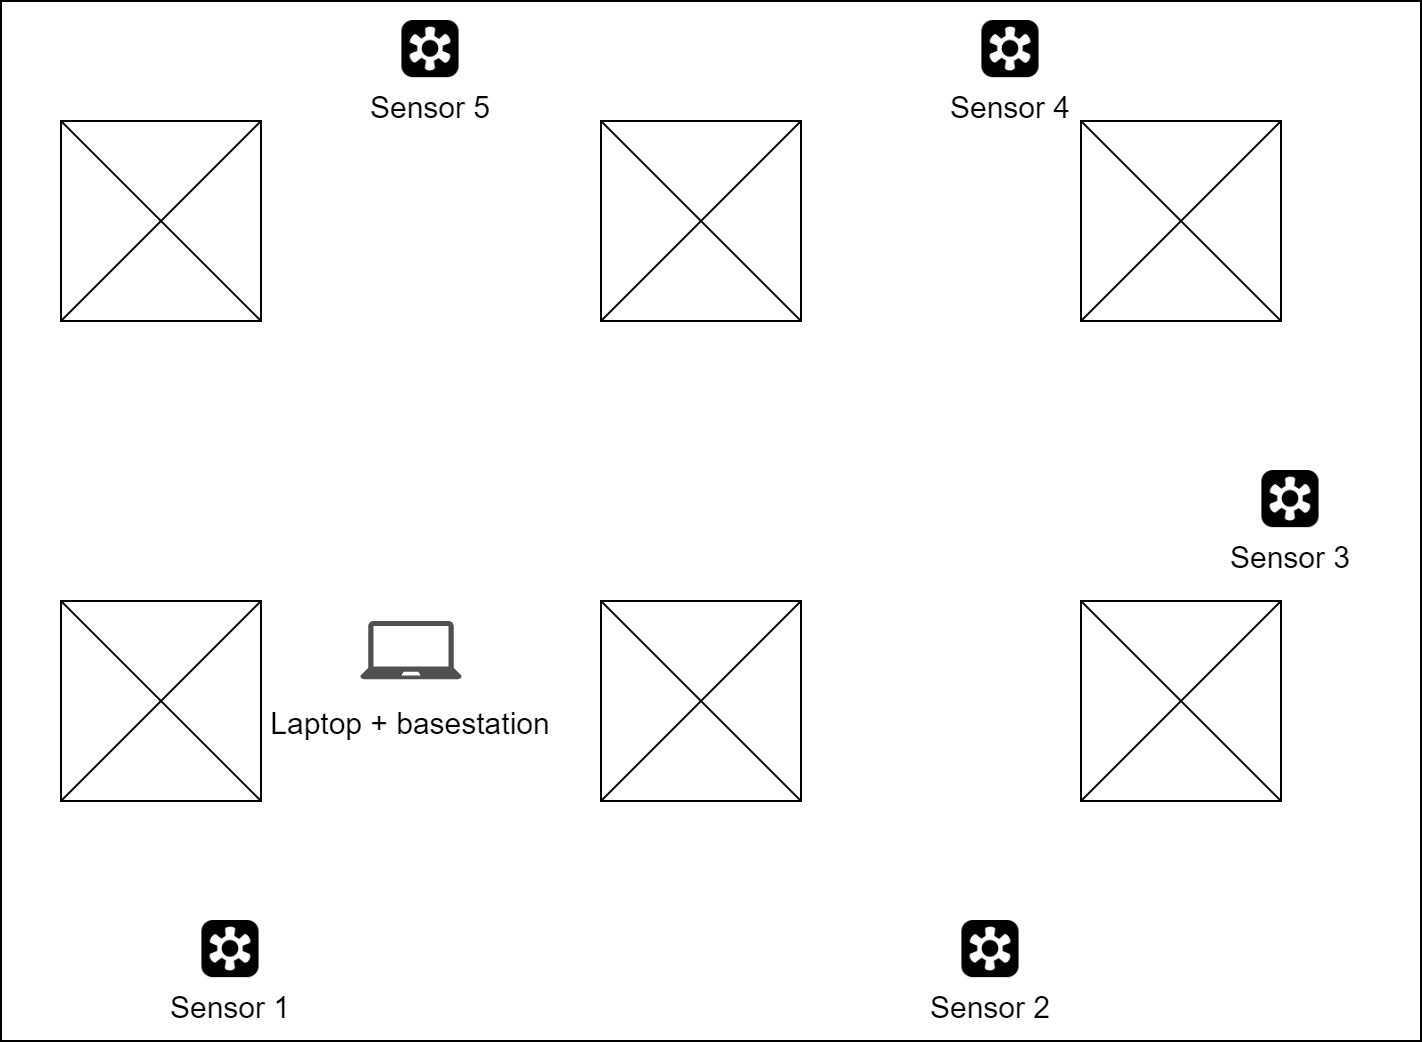
\includegraphics[scale=0.3]{Gambar/Hasil Sensing/Pengujian-Star Rooftop.jpg} 
	\caption[Denah peletakan sensor node dengan topologi tree]{Denah peletakan sensor node dengan topologi tree}
	\label{fig:denah_star_rooftop} 
\end{figure}

\begin{figure}[H] 
	\centering  
	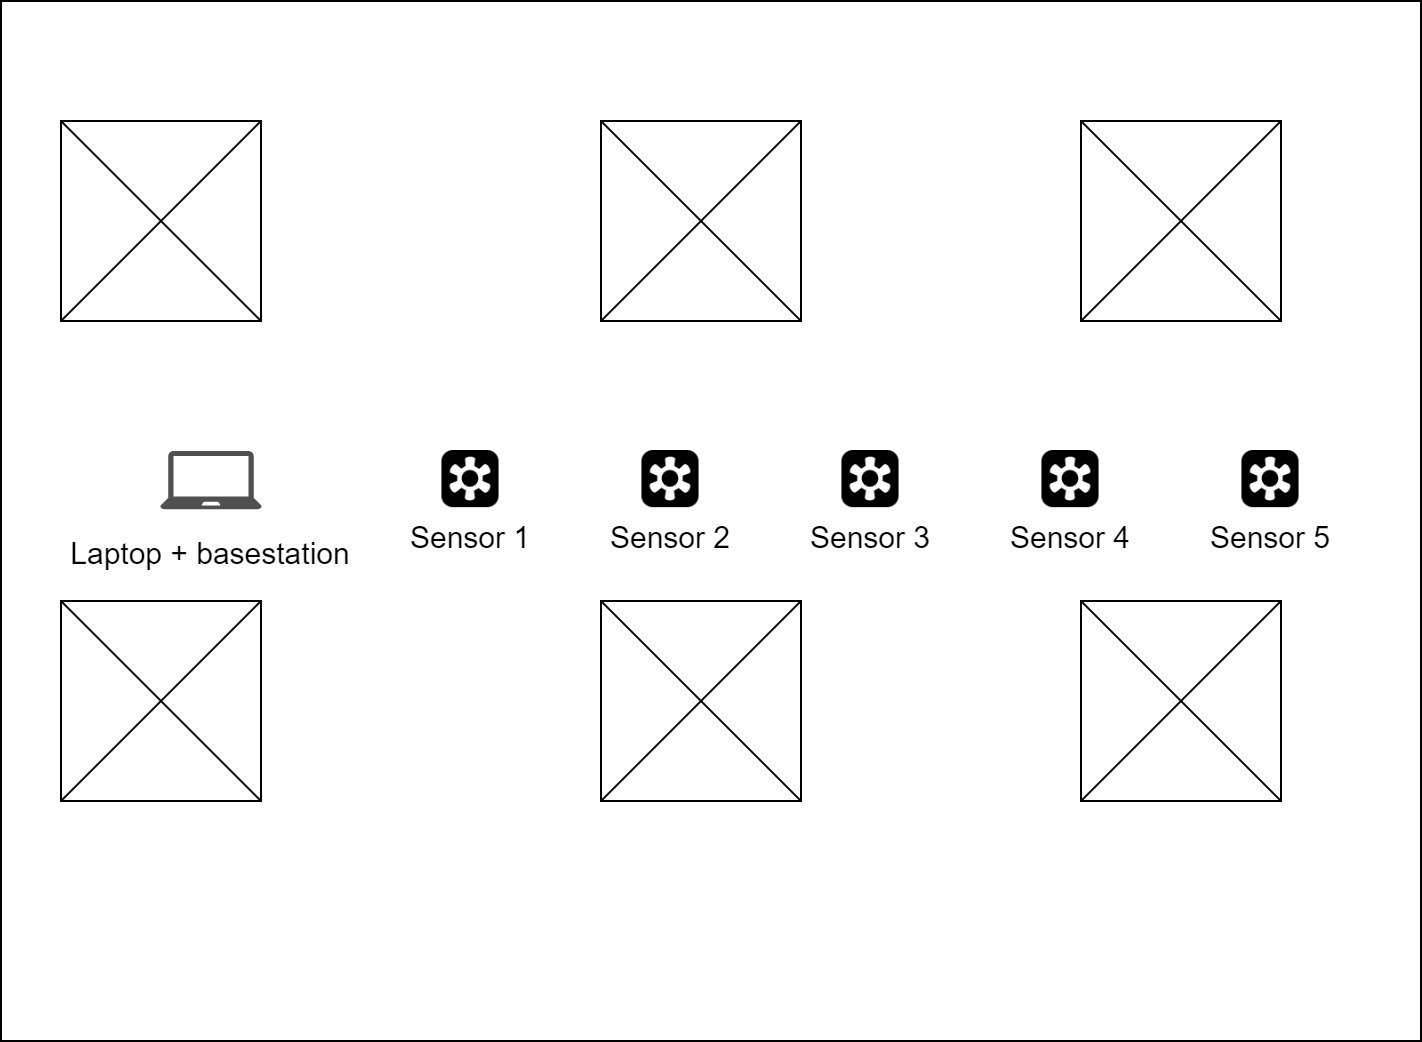
\includegraphics[scale=0.3]{Gambar/Hasil Sensing/Pengujian-Tree Rooftop.jpg} 
	\caption[Denah peletakan sensor node dengan topologi tree]{Denah peletakan sensor node dengan topologi tree}
	\label{fig:denah_tree_rooftop} 
\end{figure}

Pengujian dilakukan saat siang hari dengan cuaca berawan. Hasil grafik dari pengujian dapat dilihat pada lampiran \ref{lamp:C}.

\begin{itemize}
    \item Topologi star
    
    \begin{table}[H]
	\centering
	\caption{Tabel hasil getaran yang tertangkap di Rooftop gedung 10 dengan topologi star}
	\label{tree_paskal_tabel}
    	\begin{tabular}{|p{2cm}|p{2cm}|p{3cm}|p{3cm}|p{3cm}|}
    		\hline 
    		Id Sensor & Waktu & Frekuensi pada sumbu $x$ (Hz) & Frekuensi pada sumbu $y$ (Hz) & Frekuensi pada sumbu $z$ (Hz) \\
    		\hline
    		SensorA & 10:37:15 & 0.32 & 0.40 & 1.40 \\
    		\hline
    		SensorB & 10:36:33 & 0.12 & 0.12 & 1.07 \\
    		\hline
    		SensorC & 10:35:22 & 0.10 & 0.09 & 1 \\
    		\hline
    		SensorD & 10:35:40 & 0.10 & 0.07 & 1.05 \\
    		\hline
    		SensorE & 10:36:29 & 0.18 & 0.10 & 0.99 \\
    		\hline
    		SensorA & 10:37:19 & 0.30 & 0.40 & 1.35 \\
    		\hline
    		SensorB & 10:36:42 & 0.10 & 0.10 & 1.05 \\
    		\hline
    		SensorC & 10:35:40 & 0.09 & 0.09 & 1.05 \\
    		\hline
    		SensorD & 10:35:54 & 0.12 & 0.05 & 0.95 \\
    		\hline
    		SensorE & 10:36:38 & 0.18 & 0.10 & 1 \\
    		\hline
    		SensorA & 10:37:23 & 0.29 & 0.35 & 1.35 \\
    		\hline
    		SensorB & 10:36:50 & 0.12 & 0.10 & 1.05 \\
    		\hline
    		SensorC & 10:35:46 & 0.1 & 0.1 & 1 \\
    		\hline
    		SensorD & 10:36:08 & 0.13 & 0.06 & 1.02 \\
    		\hline
    		SensorE & 10:36:47 & 0.18 & 0.10 & 1.1 \\
    		\hline
    	\end{tabular}
    \end{table}
    
    \item Topologi tree
    
    \begin{table}[H]
	\centering
	\caption{Tabel hasil getaran yang tertangkap di Rooftop gedung 10 dengan topologi tree}
	\label{tree_paskal_tabel}
    	\begin{tabular}{|p{2cm}|p{2cm}|p{3cm}|p{3cm}|p{3cm}|}
    		\hline 
    		Id Sensor & Waktu & Frekuensi pada sumbu $x$ (Hz) & Frekuensi pada sumbu $y$ (Hz) & Frekuensi pada sumbu $z$ (Hz) \\
    		\hline
    		SensorA & 15:27:17 & 0.05 & 0.07 & 1.08 \\
    		\hline
    		SensorB & 15:27:30 & 0.10 & 0.19 & 1.05 \\
    		\hline
    		SensorC & 15:27:47 & 0.13 & 0.12 & 1.13 \\
    		\hline
    		SensorD & 15:28:17 & 0.09 & 0.13 & 0.90 \\
    		\hline
    		SensorE & 15:28:27 & 0.12 & 0.1 & 1.01 \\
    		\hline
    		SensorA & 15:27:26 & 0.05 & 0.07 & 1.05 \\
    		\hline
    		SensorB & 15:27:41 & 0.11 & 0.17 & 1.3 \\
    		\hline
    		SensorC & 15:27:58 & 0.13 & 0.13 & 1.1 \\
    		\hline
    		SensorD & 15:28:28 & 0.10 & 0.13 & 0.92 \\
    		\hline
    		SensorE & 15:28:39 & 0.12 & 0.12 & 1 \\
    		\hline
    		SensorA & 15:27:35 & 0.06 & 0.09 & 1.08 \\
    		\hline
    		SensorB & 15:27:52 & 0.11 & 0.17 & 1 \\
    		\hline
    		SensorC & 15:28:09 & 0.13 & 0.13 & 1.15 \\
    		\hline
    		SensorD & 15:28:39 & 0.1 & 0.13 & 0.90 \\
    		\hline
    		SensorE & 15:28:50 & 0.1 & 0.1 & 1.02 \\
    		\hline
    	\end{tabular}
    \end{table}
\end{itemize}

Kesimpulan yang didapatkan dari hasil pengujian di Rooftop Universitas Katolik Parahyangan adalah frekuensi tertinggi pada sumbu x adalah 0.32 Hz di SensorA pada pengujian topologi star dengan waktu 10:37:15. Frekuensi tertinggi pada sumbu y adalah 0.40 Hz di SensorA pada pengujian topologi star dengan waktu 10:37:15 dan 10:37:19. Frekuensi tertinggi pada sumbu z adalah 1.40 di SensorA pada pengujian topologi star dengan waktu 10:37:15.

\pagebreak
\subsection{Kesimpulan Hasil Pengujian}
Berdasarkan pengujian yang telah dilakukan pada dua tempat yaitu Mall Paskal 23 Square dan Gedung Rooftop Universitas Katolik Parahyangan, didapatkan kesimpulan nilai frekuensi yang ditangkap berbeda diantaranya karena keramaian dari kedua juga berbeda. Frekuensi terendah yang tercatat selama proses pengujian adalah 0.05 Hz pada pengujian di Mall Paskal 23 Square topologi star oleh SensorA dengan waktu 16:48:40. Frekuensi tertinggi yang tercatat slama proses pengujian adalah 2.4 Hz pada pengujian di Mall Paskal 23 Square topologi star oleh SensorA dengan waktu 15:07:28 

\subsection{Masalah dalam pengujian}
Berikut masalah-masalah yang dihadapi saat melakukan pengujian:

\begin{enumerate}
    \item Sensor node yang digunakan untuk melakukan pengujian terbatas, sehingga sensor node harus dipakai secara bergantian dengan mahasiswa lain yang mengambil topik skripsi yang berkaitan dengan sensor node.
    
    \item Saat pengujian, sensor node dapat mati secara tiba-tiba, karena sumber power sensor node yaitu baterai dapat habis saat sensor node melakukan \textit{sensing}
    
    \item Cuaca hujan yang menghambat pengujian karena pengujian dilakukan di ruangan semi terbuka.
    
    \item Pengujian dilakukan saat adanya pandemi Covid19, sehingga adanya keterbatasan untuk penggunaan sensor node secara bersama dengan mahasiswa lain yang memilih topik skripsi yang berkaitan demi mematuhi aturan protokol kesehatan.
\end{enumerate}